\documentclass[12pt, a4paper, english]{report}

\usepackage{fyp}

\author{
  Dara MacConville | 17377693\\[0.5em]
  {\small A thesis submitted in partial fulfilment of the requirements for the \\ B.Sc. Computational Thinking\\[0.5em]}
  {\small 5 Credits\\[0.5em]}
  {\small Advisor:\hspace{2mm}Dr. Philippe Moser}
}

\affil{Department of Computer Science\\Maynooth University, Ireland}

\date{April 13, 2019}


\begin{document}

  \maketitle

  \begin{abstract}
      The goal of this project was to formalise and implement alternative models of computation inside the proof assistant Isabelle,
      and then to make use of this to assist in providing definitions on and proving various results about these models.
      In particular it focuses on Cellular Automata,
      in both one and two-dimensional variants, and with differing topologies.
  \end{abstract}

  \setcounter{tocdepth}{1}

  %% We'd like all lists to appear as sections in one big chapter.

  \tableofcontents
  \thispagestyle{empty}

  \chapter*{Lists of Floats}

  \listoftables

  \listoffigures

  \lstlistoflistings
  \thispagestyle{empty}


  \setcounter{page}{0}
  \chapter{Introduction}
% TODO references for these
Cellular Automata (CA) are a very simple model of computation.
There are many variations and extensions of them,
and some like Conway's Game of Life and Rule 110 are known to be Turing Complete.
Isabelle is a proof assistant that can be used for anything from mathematical proofs to formal verification of software properties.


\section{Topic addressed in this project}

This project looks at formalising models of Cellular Automaton in Isabelle to help deal with the complexity that comes with trying to mathematically prove results about them.
In addition to providing a formalisation of six different variants of CA,
this project provides definitions of important properties they may have, and proves some lemmas and theorems necessary to work with them.


\section{Motivation}

It can be very difficult to work with high level concepts while still being rigorous,
and theoretical Computer Science is a very abstract and mathematical discipline that requires exactly that.
One of the main concepts used in theoretical CS is the Turing Machine.
While it provides an excellent way of approaching computation that allows for conceptually easy high level proofs,
being very strict and formal in these can prove difficult.

However the Turing Machine is not the only available model in CS.
One of the goals of this project was to look at \emph{alternative} concepts that achieve the same thing,
to help better appreciate the benefits and drawbacks.
Cellular Automata were chosen as they strike a good balance between simplicity and complexity,
as they have a very simple idea, 
but come with additional geometric aspects to consider.

The motivation to use a proof assistant rather than traditional pen and paper proofs
comes from a desire to use the exactness of computers to cope with issues that stem from highly layered and detailed concepts.


\section{Approach}

\docs{Isabelle} was chosen as the language and framework to implement these models in.
This is due to it being very high level,
and having advanced tools available to ease the creation process.
These include the multitool command \mintinline{isabelle}{sledgehammer} which invokes several Automatic Theorem Provers and Satisfiability-Modulo-Theories solvers, and \mintinline{isabelle}{nitpick} which provides counter-examples to statements.
% TODO put links to docs on sledgehammer/nitpick
These take the burden of large manual proofs off the programmer,
while still encouraging simple and understandable definitions,
as these are more easy to automatically prove results on.

Isabelle also has a powerful and expressive type system,
and the decision was taken to directly make use of this in the CA definitions created.
This involved making each kind of CA explicitly into a type,
to make use of automatic type checking and other benefits.
This contrasts with a more mechanical approach taken in a paper \cite{urban} that also works on implementing Turing Machines and other computability concepts in Isabelle.
One reason for this difference in approach is their work involves the need to convert between different models, for instance Abacus Machine to Turing Machine,
whereas in this project no conversions are done.
Additionally the design of such ``machines'' lend themselves to being built in such a way.
However it was not possible to entirely avoid that way of thinking with CA either, in particular in the two dimensional case.


\section{Metrics} \label{sec:metrics}

It can be difficult to evaluate exactly how well a definition has been translated from the informal to the formal.
It could be possible to have a very precise and elegant program that doesn't actually capture the intuitive content of the informal idea.
As such the definitions written here were evaluated in two main ways:

\begin{enumerate}
    \item Understanding: Does reading the program lead to the same understanding as reading the original definitions?
        If so then it is capturing the same spirit as the original,
        even if the means of execution may differ slightly or significantly.
    \item Functionality: As CA are systems that can be run,
        it is necessary to run them on example programs and see the correct results are achieved.
        Speed is not a trait that is sought out but accuracy is of course essential.
\end{enumerate}

Also taken into account is the ability to state properties of these systems,
and the ease or difficulty of proving results about them.



%\begin{figure}[h]
%    \centering
%    \includegraphics[scale=0.7]{blinkers_both.pdf}
%    \caption{Both forms of a Blinker}
%    \label{fig:binkers}
%\end{figure}

%\begin{myminted}{Some Example Isabelle}{testcode}
%    fun garden_of_eden :: "CA ==> bool" where
%    "garden_of_eden (CA s r) = (¬(EX s0. (CA s0 r) yields s))"
%
%    theorem "ca yields State (run ca 1)"
%    proof-
%      show ?thesis using yields_def by blast
%    qed
%\end{myminted}

  \chapter{Technical Background}

\section{Topic Material}

\subsection{Formalisations in Computability Theory}

As mentioned before,
this is certainly not the first formalisation of computability theory concepts inside of proof assistants.
Other works however have focused on more traditional models or with certain specific proofs in mind.
These include $\lambda$-calculus in Coq \cite{forster},
partial recursive functions in Lean \cite{carneiro},
and the aforementioned Turing and Abacus machines in Isabelle \cite{urban}.
Other than choices of model and language,
the key difference between those works and this project is the end goal.
The three mentioned above all set about to formalise computability theory from the perspective of their chosen model or models.
This project works with just Cellular Automata and what results can be specifically shown about them.

Additionally the approach in \cite{urban} often involves specifying certain exact indices in lists and having to manipulate these numbers.
This obviously has its technical benefits and is necessary when working with TMs,
but the desire in this work was to take a ``wholemeal'' functional programming approach to the construction where possible.

The existing research that comes closest to both the goals and execution of this project,
is a formalisation of CA in Coq for the purposes of verifying a result about the firing squad problem \cite{firing}.
Their work bases the CA over the naturals $\mathbb{N}$,
and includes an explicit time parameter.
As well as that,
their transition function is based more around individual cells,
and the properties they define are all based around eventually deriving the proof.


\subsection{Cellular Automata}
The concept of CA has been around since the 1940s and were popularised in the 70s with Conway's Game of Life.
However a lot of the names and terminology associated with them comes from Stephen Wolfram \cite{wolfram}.
His work is not entirely formal,
but others have provided their own formalisations of definitions he put forward \cite{yu}.
This was especially useful as an aid in translating the some of the classifications of CA into Isabelle, 
even if their formalisation differed in many other ways.


\section{Technical Material}

\subsection{Cellular Automata}

A Cellular Automaton in general consists of a rectangular grid of cells sitting in some finite dimension,
with each one of these cells in one of a finite number of different states.
Each cell has a neighbourhood
and a rule that determines how a cell changes with each time step,
based off its own state and the states of the cells in its neighbourhood.

All the CA this project is concerned with have cells in one of only two binary states: \mintinline{isabelle}{One} or \mintinline{isabelle}{Zero}.
On diagrams \mintinline{isabelle}{One} is indicated by a filled in black square,
and \mintinline{isabelle}{Zero} by a white square.
In one dimension these are known as \emph{elementary cellular automata}.

This project deals with both one and two dimensional cellular automata.
In the one dimensional case the overall state of the whole automaton can be thought of as a single line of cells,
and in the two dimensional case as cells tiling the plane.
Extensions to higher dimensions are of course possible but not dealt with here.

The neighbourhood used for one dimensional CA here is the simplest possible,
consisting only of a trio of cells including the cell itself in the middle, and the cell to its immediate left and right as seen in \Cref{fig:nbhd_1D}.


\begin{figure}[h]
    \centering
    \includegraphics[scale=1.7]{neighbourhood_1D.pdf}
    \caption{Neighbourhood of the {\color{blue} blue} cell includes itself and the cells in {\color{red} red}}
    \label{fig:nbhd_1D}
\end{figure}

In two dimensions there are more possible neighbourhoods that still seem natural.
The one used \Cref{fig:moore} is known as the \emph{Moore neighbourhood},
made up of the nine cells that form a square including the cell itself as the centre.
Alternatives include the \emph{von Neumann neighbourhood},
which only takes the squares in the cardinal directions from the centre.


\begin{figure}[h]
    \centering
    \includegraphics[scale=1.7]{neighbourhood_moore.pdf}
    \caption{Moore neighbourhood}
    \label{fig:moore}
\end{figure}

The development of a one dimensional CA over time is best represented by multiple rows of cells,
with each new row representing the state at the next time step,
with time increasing downwards along the y-axis.
It is important to remember that the whole structure depicted never exists at any point in time,
only the one dimensional slices across.

\begin{figure}[h]
    \centering
    
\includegraphics[scale=1.7]{rule26.pdf}
    \caption{Rule 26 traces a Sierpi\'{n}ski triangle over time}
    \label{fig:rule26}
\end{figure}

A two dimensional CA is shown as a cell diagram in the plane,
with changes over time indicated via multiple diagrams adjacent to each other
and time flowing forward from left to right.

\begin{figure}[h]
    \centering
    
\includegraphics[scale=1.7]{glider.pdf}
    \caption{3 steps of a ``glider'' in Game of Life}
    \label{fig:glider}
\end{figure}

Rules can be specified by a mathematical formulation based on the cells in a neighbourhood as they are in the Game of Life,
or just explicitly defined by listing all inputs and outputs.
For elementary CA the rule is derivable from its Wolfram code which is also used as the name of the rule e.g. Rule 110.
However in this project explicit representations were used.
As an example part of the definition of Rule 110 is given in \Cref{table:rule110}

\begin{table}[htbp]
    \centering
    \begin{tabular}{c|ccc}
        % \hline
        Neighbourhood & $\blacksquare \blacksquare \blacksquare$ & $\blacksquare \blacksquare \square$ & $\blacksquare \square \blacksquare$  \\
         \hline
         Output & $\square$ & $\blacksquare$ & $\blacksquare$
        %  \hline
    \end{tabular}
    \caption{Rule 110}
    \label{table:rule110}
\end{table}


\subsection{Isabelle}

Isabelle as a proof assistant allows us to to define algebraic datatypes and pure total recursive functions,
using pattern matching, guards, and conditionals in a syntax very similar to Haskell's.
Function types are represented in the usual currying friendly way for multiple arguments.
For instance see \Cref{code:example_fun} below.

\begin{myminted}{Functions demonstrating multiple arguments and pattern matching}{example_fun}
    fun get_cell :: "state => int => int => cell" where
    "get_cell s x y = s!(nat x)!(nat y)"

    fun apply_nb :: "(cell => cell) => neighbourhood => neighbourhood" where
    "apply_nb f (Nb a b c) = Nb (f a) (f b) (f c)"
\end{myminted}

On top of these we can state and prove theorems using all the usual first order logic connectives, quantifiers and operators,
along with some Isabelle specifics.
There are multiple ways of writing proofs in Isabelle,
with some being written in the more human-readable Isar language
and others simply being a chain of commands to apply.
Both kinds will be made use of in the project.

\begin{myminted}{An example statement of theorem named ``t1'' along with proof}{example_thm}
    theorem t1 :"n>0 ==> ca yields State (run ca n)"
      apply(simp add: yields_def)
      apply(rule exI)
      apply(rule conjI)
      apply(auto)
      done
\end{myminted}

Strictly speaking everything in quotation marks is part of HOL,
the logic that Isabelle runs on by default,
and the language in which most of the actual programming happens.
However for the sake of simplicity throughout this report the whole language and infrastructure shall simply be referred to as ``Isabelle''.
Each file in Isabelle is referred to as a \mintinline{isabelle}{theory},
and is a selection of definitions and proofs.
These theories may draw in and reference other predefined or user made theory files as dependencies in the same way as any programming language uses libraries.

  \chapter{The Problem}

\section{Problem Analysis}

The goal of the project was to somehow implement a variety of types of CA in Isabelle in a workable fashion.
The types of CA were one or two dimensional CA that were either finite or infinite,
leading to essentially four main categories to develop.
There were two main issues to address for each of these.

The first was how to implicitly or explicitly represent the state of a CA.
This question was especially key in the infinite case, 
as it requires thinking beyond traditional finite data structures.
The other topic of interest was how to develop the state of the CA as time progresses.
Again this is much more a difficult and important issue in the infinite case,
as you cannot simply apply a function over infinitely many values.
This rules out the obvious choices such as using \mintinline{isabelle}{map} and other functions in a similar vein.

The finite automata also had certain issues that do not occur in the infinite cases.
As they are finite they have boundaries,
and for cells on these boundaries the neighbourhood necessary to determine its evolution does not exist in the standard way.
This requires a decision to be made to either adjust the neighbourhood of these cells,
or the rule that applies to them.

  \chapter{The Solution}

The purpose of this chapter is to clearly identify, discuss, and justify the decisions you make
Depending on your type of project, you may not need to include all of these:


\section{Architectural Level}

\begin{figure}[h]
    \centering
    \includegraphics[scale=0.62]{session_graph.pdf}
    \caption{Dependency graph of project Theories}
    \label{fig:graph}
\end{figure}

\Cref{fig:graph} represents the overall architecture of dependencies of the various theory files in the project,
with files further down the tree depending on those above.
\mintinline{isabelle}{[Pure]} and \mintinline{isabelle}{[HOL]} contain the base definitions necessary to do work in Isabelle,
all the rest are new theories created for the project.

From the simplest core definitions given in \mintinline{isabelle}{CA_Base},
the project essentially splits into two due to the differences in implementing one dimensional versus two dimensional CA.
However the internal structure of these two subtrees are exactly the same apart from the distinction in dimension.
They both contain a base file for the two kinds of finite CA,
and another file dealing with the infinite case.

Each of the six root nodes contains the definition of one of the six distinct kinds of CA realised in the project.
They very roughly increase in power and complexity from left to right.

\section{The Cellular Automata Type}

The type of \mintinline{isabelle}{Cellular Automata} is redefined for each of the four main branches in the project.
Those are elementary finite,
two-dimensional finite,
elementary infinite,
and two-dimensional infinite.
This is due to the geometric and functional differences that have to exist in the \mintinline{isabelle}{state} type parameter underlying each broad class of CA.
Despite this, the actual signature of the type remains unchanged for each.
This is the allow the definitions and proofs that sit on top of them to make the same assumptions about type structure and composition.
As shown below in \Cref{code:ca_def} the definition is very compact and simple.
All CA also share the binary cell type given in \Cref{code:cell_def}.

As you would hope,
a Cellular Automata consists only of the current global state it is in,
and the rule necessary to transition it to the next state.
This however does hide quite a lot of complexity,
and in fact the actual functioning of a CA is created from more than these two parameters.

As an example of this,
\cite{yu} actually defines CA as a 4-tuple $(k, S, N, f)$,
where $k$ is the dimension,
$S$ the set of states,
$N$ the neighbourhood,
and $f$ the local rule.
This is certainly more transparent then the definition given here.
In this project's version the information about neighbourhoods is given implicitly from a neighbourhood function that sits in the local context where we want to actually run the CA.
The reason for the approach taken here is for elegance and ease of use in further results on the CA type.
Adding more information to the type directly can mean more work in pattern matching,
and constructing and deconstructing the type every time it is used.

\begin{myminted}{Cell definition}{cell_def}
    datatype cell = Zero | One
\end{myminted}

\begin{myminted}{CA type signature}{ca_def}
    datatype CA = CA (State : state) (Rule : rule)
\end{myminted}

The \mintinline{isabelle}{State} and \mintinline{isabelle}{Rule} that are capitalised are just syntactic sugar for defining accessor functions for those arguments to the type.
So the \mintinline{isabelle}{State} function takes a CA and returns its state, 
and similar for \mintinline{isabelle}{Rule}.

It is also worth noting that the CA here is not directly defined as a tuple.
Using a unique datatype carries more semantic weight then giving a \mintinline{isabelle}{type_synonym} to a tuple.
The same concept does not exist in general mathematics so purely mathematical approaches to formalisms usually just involve a tuple.


\subsection{State}

As mentioned in the above paragraphs,
the \mintinline{isabelle}{state} type is designed differently across the four general distinctions of CA.
As such the more detailed description of each is left to its own respective section.
For a high level overview it suffices to say that the finite CA states were simply a one or two dimensional list of states,
given geometry through either pattern matching or indices.
The infinite CA states were modeled completely differently,
as a function from the integers to cells.

\subsection{Neighbourhoods \& Rules}

Unlike \mintinline{isabelle}{state},
\mintinline{isabelle}{rule} is defined exactly the same way for all CA, as given in \Cref{code:rule_def}.
The only differing factor being the type of neighbourhood it acts on.

\begin{myminted}{Type definition of \mintinline{isabelle}{rule}}{rule_def}
    type_synonym rule = "neighbourhood => cell"
\end{myminted}

Neighbourhoods differ between one and two dimensions as expected but not in a conceptually deep way.
As shown in \Cref{code:nb_def} the only practical difference is adding more \mintinline{isabelle}{cell} arguments.

\begin{myminted}{The two kinds of neighbourhood}{nb_def}
    (* One dimensional *)
    datatype neighbourhood = Nb cell cell cell

    (* Two dimensional *)
    datatype neighbourhood = Nb
    (NorthWest:cell) (North:cell)  (NorthEast:cell)
    (West:cell)      (Centre:cell) (East:cell)
    (SouthWest:cell) (South:cell)  (SouthEast:cell)
\end{myminted}

\section{Finite Cellular Automata}

There ended up being two separate paths taken in dealing with the cells on the boundary of the finite CA.
The first,
which for the purposes of the project is named \emph{bounded},
is the simplest conceptually,
but not necessarily in implementation.

Bounded CA deal with the problem of determining the neighbourhood of a cell on the edge simply via ``padding''.
For the purposes 








\section{Analytical Work}

E.g. Equations, etc. that describe your solution


\section{Low Level}

E.g. Method specifications, Algorithms, etc.


\section{Implementation}

Discuss anything interesting here; put full source code in an appendix or attachment



  \clearpage % or \cleardoublepage
  \addcontentsline{toc}{chapter}{Bibliography}
  \nocite{*}
  \printbibliography

  %\input{Appendix.tex}

\end{document}
